As we discussed in \ref{chp:res}, the three features we introduced in Amodal-net \ie cascade, Soft NMS and interative mask head all boost the performance of the model. However, reprojection is not as successful as those three features. It would be interesting to discuss what is the reason.

One reason could be the distribution of objects in SAILVOS dataset. As shown in \ref{fig:sailvos_cls}, person class contribute to the largest number of objects. But objects in person class usually move between frames, which means reprojection will not align it correctly.

\begin{figure}[t]
\centering
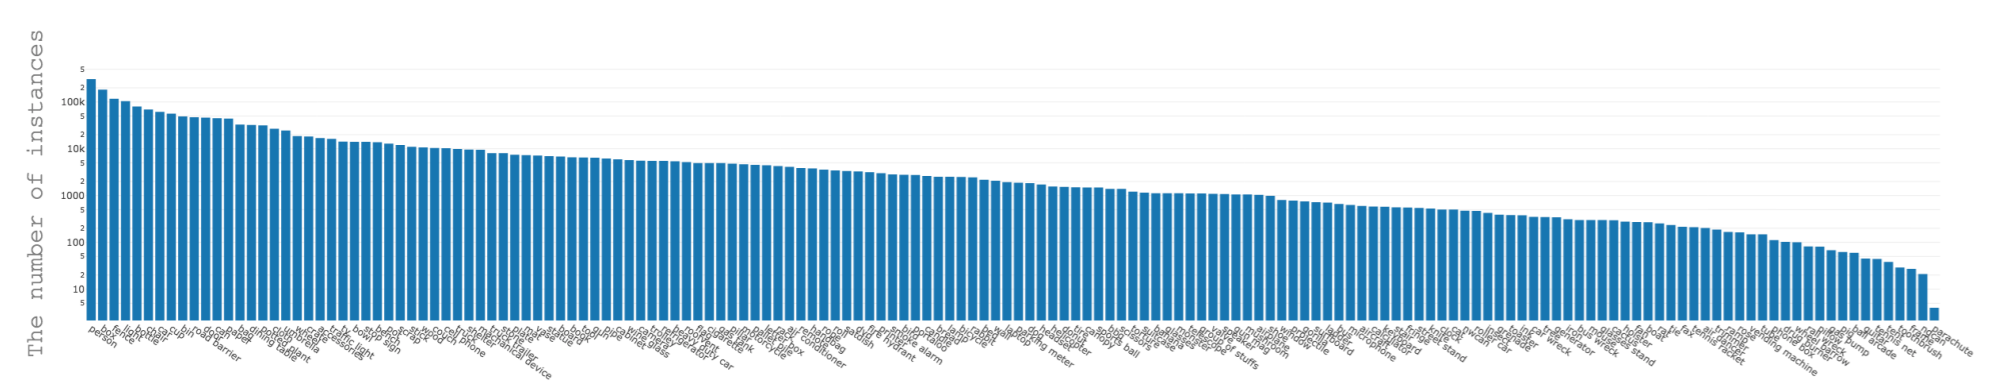
\includegraphics[scale=0.23]{fig/sailvos_cls_dist.png}

\caption{The number of instances per class in the proposed SAIL-VOS dataset. There are 162 semantic classes in total. These 162 classes are remaped to 24 COCO classes in our experiments. }
\label{fig:sailvos_cls}
\end{figure}

Another limitation is data augmentation. Experiments for Amodal-net was using augmentations such as random flip. But random flip is not compatible with reprojeciton because the camera matrices and depth map that is used in reprojection will not be correct if the image is flipped. This challenge can be solved if we modify the depth and camera metrices when flip is used, but this is not explored in this thesis due to the complications in implementation.